\subsection{\glsdesc{IBV}}

Context and institutions are the prevalent terms when it comes to \rbv and \inbv.
The lack thereof of considering institutions and context is part of the critiques in that have emerged~\cite{Narayanan:2005}.
Under certain circumstances for example, the pursuit of cost leadership can be deemed unethical in that the raising broilers however sustainable were seen as cruel by modern animal welfare standards. 
Some times the cost-leadership strategy can drive companies to engage in (illegal) price fixing actions. 
In the Dutch mobile phone market, the telecom providers (KPN, Vodafone and T-mobile) have been reprimanded twice in the last decade or so by the \gls{ACM}\fn{The \gls{ACM} is the new name for the \gls{NMA} witch is the Dutch regulatory agency for competitions, comparable tot the British \gls{OFT} (soon to be \gls{CMA}) } for price fixes deals on mobile calling costs\fn{Sourced from \url{http://www.volkskrant.nl/vk/nl/2844/Archief/archief/article/detail/3067315/2011/12/07/Mobiel-bellen-blijkt-te-duur-door-kartel.dhtml}}. \\


 
 
 %%% INSTITUTIONAL BASED VIEW EZplaing
The institutional based view dictates that firms performance and choices do not only depend on resources and the industry the firm is competing in, but also depends on the environment in which it is operating. 
This environment is the context that has been mentioned before.

%Third Leg

Context is the third leg~\cite{Peng:2009} that influences the various decisions that firms have decide on in~\ib. 
These institutions present themselves in two forms `formal' and `informal'. 
So~\ibv~takes into account not only strategic choices driven by industry conditions and firm-specific resources, that traditional strategy research emphasises (~\cite{Porter:1980,Barney:1991}), but are also a reflection of the formal and informal constraints of a particular institutional framework that decision makers confront (\cite{Oliver:1997,Scott:1995}). 

~\ibv~is supported by two forces; external and internal in nature according to~\cite{Peng:2009}. 
The latter is the institutionalism movement by the likes of economist~\cite{North:1990} and sociologist like~\cite{DiMaggio:1983,Scott:1995}. 
These institutions are known as the rules of the game.
More on the theory of institutions will be investigated in section #ref.\\

The internal forces that underpin~\gls{IBV} are a reaction to criticisms on the theory of~\gls{InBV} of a lack of awareness of context~\cite{Narayanan:2005}. 
\cite{Kraaijenbrink:2009} also summarised \gls{RBV} critiques in his 2009 paper. 
He concluded that it is mainly the definition of `resource' and `valuable' in combination with the lack of acknowledgement of the combination of bundling resources and the human involvement, that is undermining strength of \gls{RBV}.
Likewise~\cite{Priem:2001} concluded that the contexts are missing from \gls{RBV}, where~\cite{Dung:2012} states that the ``resource-based view often neglects the issues of strategy implementation, i.e., various activities through which competitive advantage is directly created. Some resources may be valuable and rare at some point in time, this can change in an instant." 
Take a look at the operating system that Nokia used in its mobile phones in the early 2000s. 
This was considered the peak of user-friendliness; until the iPhone came along. 
The rare resource of a user-friendly operating system and user interface became defacto obsolete hence non-valuable.\\

The \ibv~tries to come up with an answer to these critiques. 
Strategic literature does not discuss the specific relationship between strategic choices and institutional frameworks~\cite{Peng:2008}.
Externally, the rise of new institutionalism throughout the social sciences has energised scholarly attention in strategy to focus on how institutions matter. 
Internally, the frustration associated with the industry-based and resource-based views’ lack of adequate attention to contexts has called for new theoretical perspectives that can overcome these drawbacks. 
The result is the emergence of the institution-based view~\cite{Peng:2009} (see picture~\ref{fig:Peng2000}).
%\begin{figure}[htbp!]
%	\centering
%	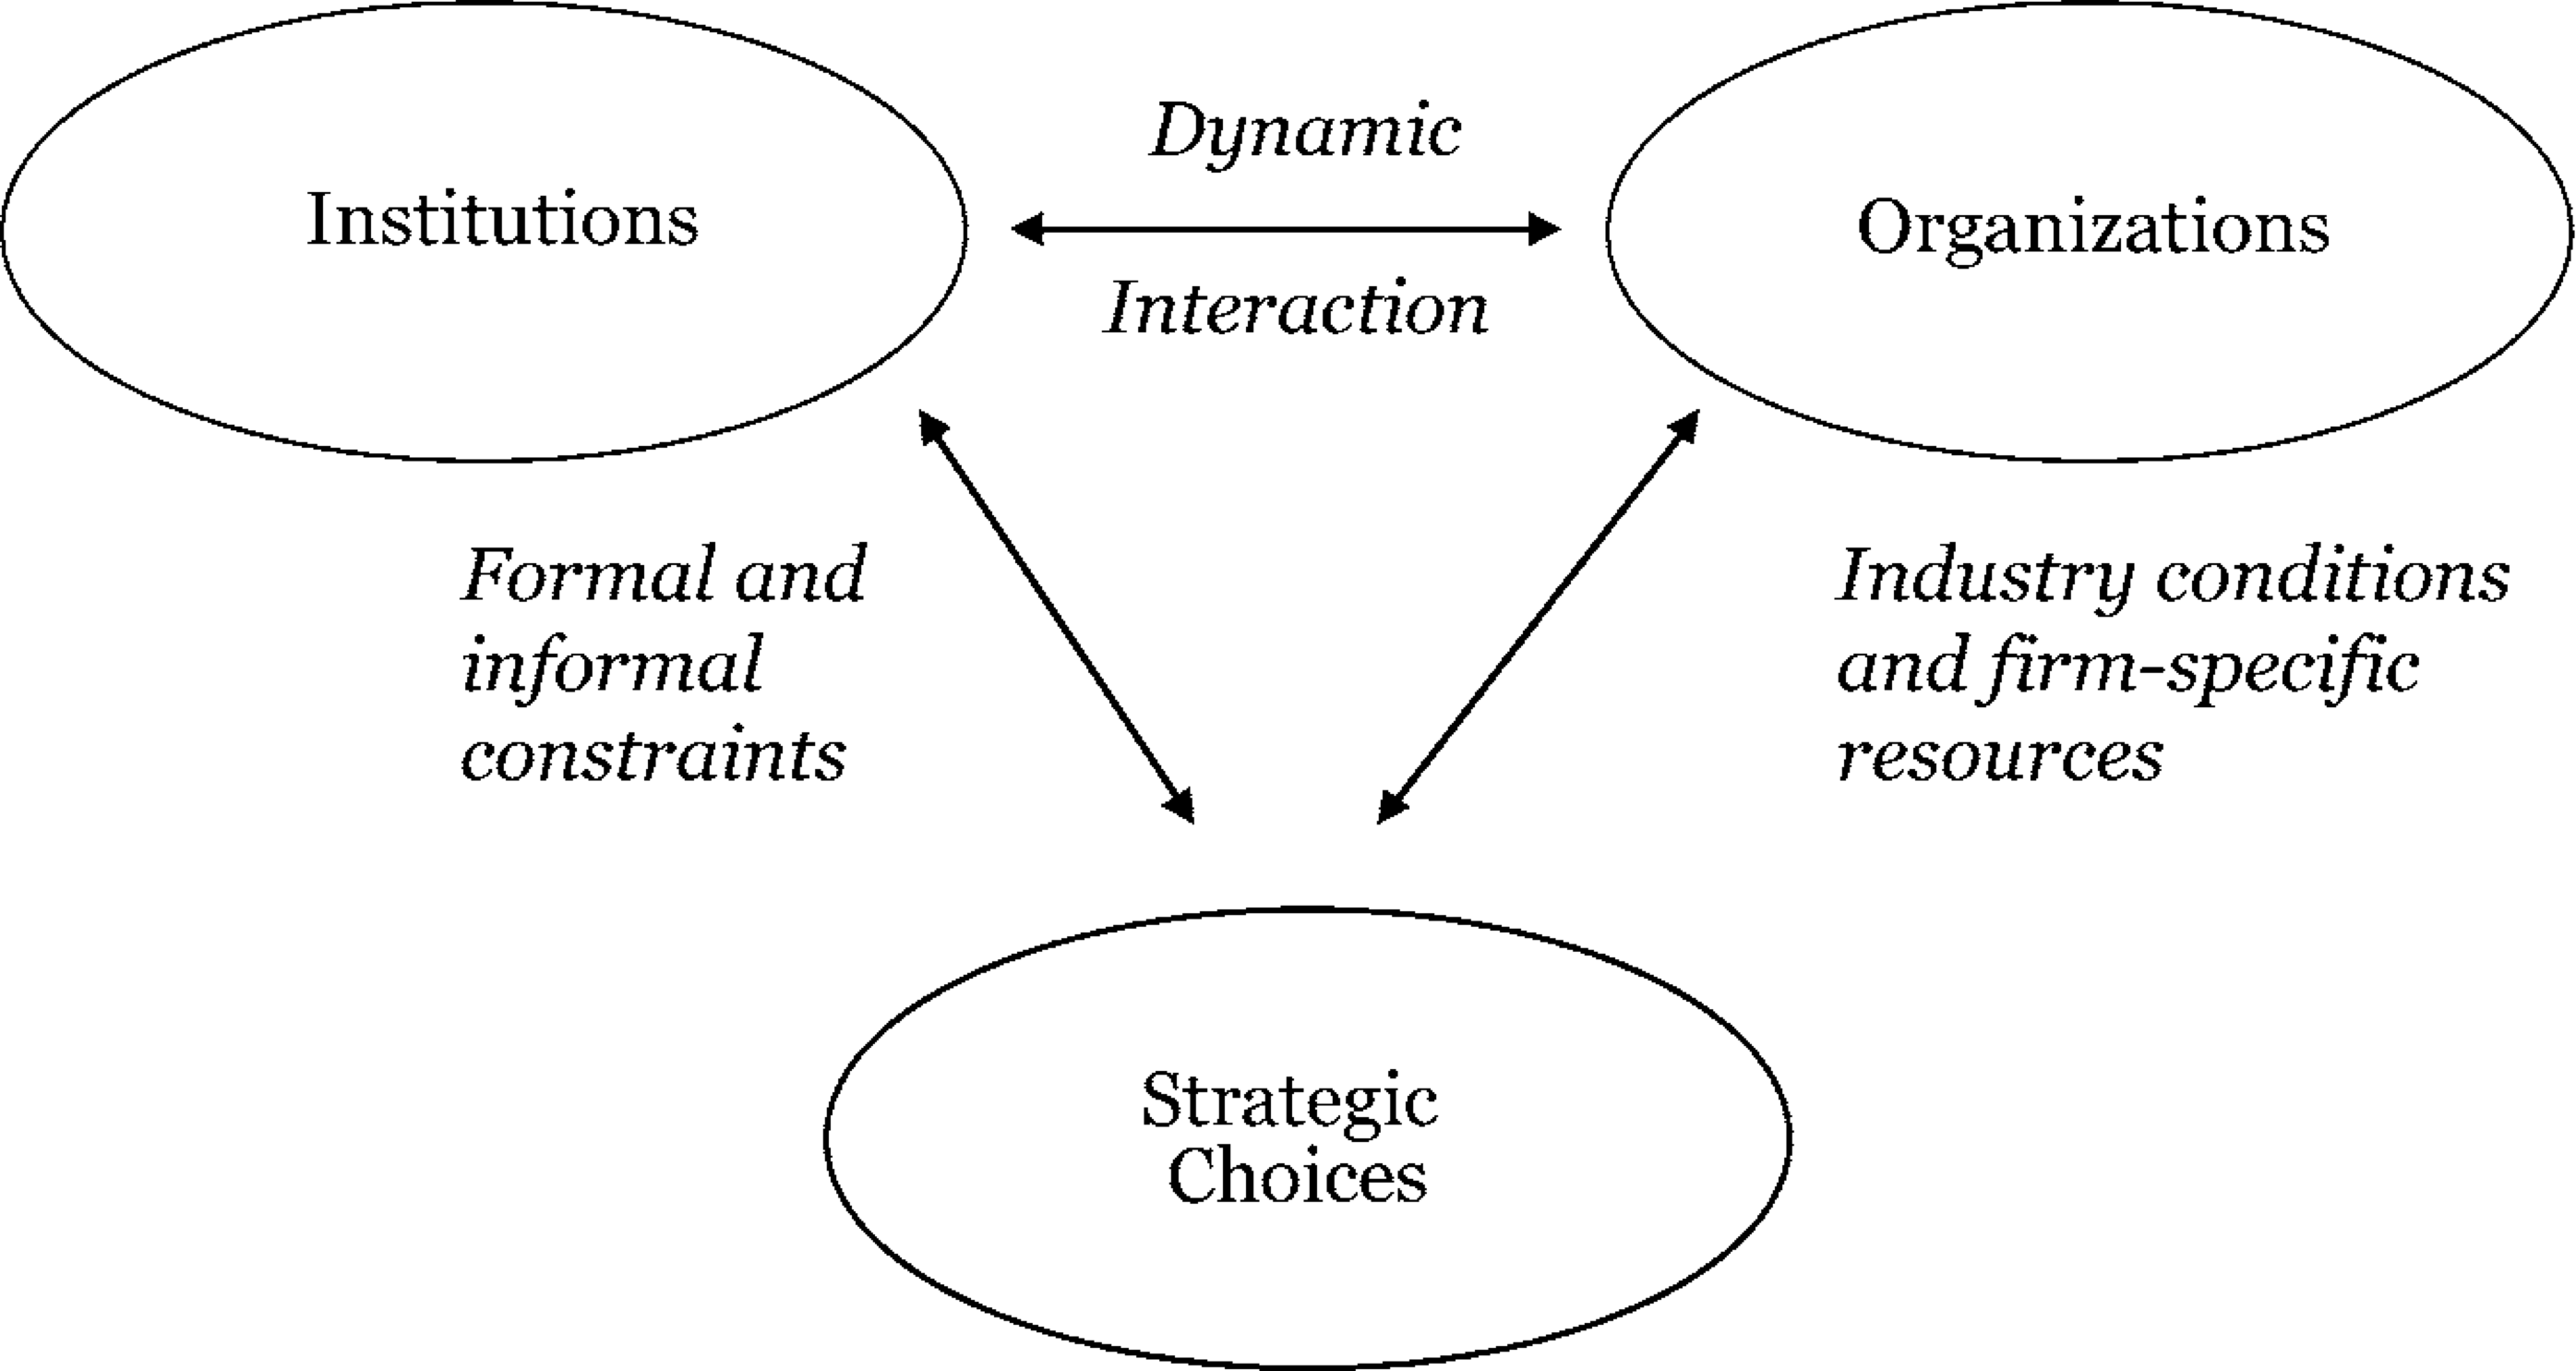
\includegraphics[width=0.65\textwidth]{IBV.png}
 %	\caption{Institutions, organisations, and strategic choices. Source:~\cite{Peng:2000}}
% 	\label{fig:Peng2000}
%\end{figure}

\begin{figure}[h]

\centering
\begin{tikzpicture}
% STYLES
\tikzset{
    ellips/.style={ellipse, minimum width=100pt,
    align=center,node distance=3cm,inner sep=5pt,text width=2.5cm,minimum    
    height=2.0cm,>=stealth'}%fill=black!10
}

\node [ellips](Choices) {Strategic Choices};
\node [above=2cm of Choices](dummy) {};
\node [ellips, force, left=1.5cm of dummy] (Institutions) {Institutions};
\node [ellips, force, right=1.5cm of dummy,drop shadow,draw] (Organisations) {Organisations};

% Draw the links between 
\path[<->,thick] 
   (Choices) edge node[anchor=center, text width=3.5cm, below left, midway] {Industry conditions and 
    firm-specific resources}  (Institutions) 
   (Choices) edge node[anchor=center, text width=3.5cm, below right, midway] {Formal and informal 
   constraints} (Organisations)
 (Institutions) edge  node [midway, below] {interaction} node[midway, above] {Dynamic} (Organisations);

\end{tikzpicture} 
\label{fig:Peng2000} 
\caption{Institutions, organisations, and strategic choices. Source:~\cite{Peng:2000}}%
\end{figure}



This figure (\ref{fig:Peng2000}) shows the dependance on both the theories of~\cite{Barney:2001} and~\cite{Porter:1980} for~\ibv. Obviously~\ibv is not an attempt to dismiss other theories more an attempt to complete theories on strategy as they exist at the moment. Strategy is about making the right choices at the correct moment. \\

Given the influence of institutional frameworks on firm behaviour, any strategic choice that firms make is inherently affected by the formal and informal constraints of a given institutional framework (\cite{North:1990,Oliver:1997}). 




Treating institutions as independent variables, an institution-based view on business strategy, therefore, focuses on the dynamic interaction between institutions and organisations, and considers strategic choices as the outcome of such an interaction (see figure~\ref{fig:ibv})\cite{Peng:2002}.
Not only have more scholars come to realise that institutions matter~\cite{Powell:1991,Scott:1995}, but also that strategy research cannot just focus on industry conditions and firm resources.~\cite{Khanna:1997}\\

%Uitleg INstitution Based View
These are the formal and informal rules of the game~\cite{North:1990}. 








When markets work smoothly in developed economies, ``the market-supporting institutions are almost invisible".~\cite{McMillan:2007}

The effect of institutions on strategy can be seen most obviously in the asian economies~\cite{Peng:2002}.




\begin{figure}[htbp!] 
      \label{fig:Peng2009}
	\centering
	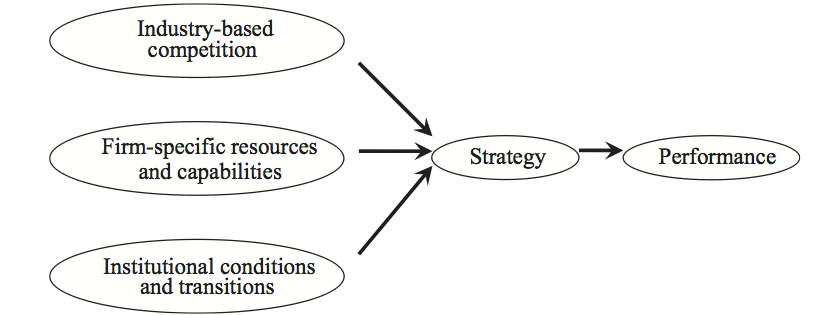
\includegraphics[width=0.65\textwidth]{Peng2009.png}
 	\caption{The Institution-Based View as a Third Leg for a Strategy Tripod. Source:~\cite{Peng:2009}}
\end{figure}









These institutions are influencing the decision making process in~\gls{IB}.  The dynamic that takes place is depicted in picture~\ref{fig:ibv}. 


So~\ibv is cannot consist by itself but needs \rbv~\cite{Barney:1991, Porter:1980} as is shown in figure~\ref{fig:ibv}. 
Where \rbv looked solely at the firm in a set environment \ibv also takes the surroundings into account. These surroundings are the institutions that govern the environment the \mne is playing the game. 
The actions of institutions can be divided into three pillars. Compliance from the firms occurs through \\(1) expedience (regulative pillar or coercive \iso),\\
 (2) social obligation (normative pillar or normative \iso), or \\
 (3) on a taken for granted basis (cognitive pillar) or mimetic \iso~where organisations respond to uncertainty by adopting patterns of other organisations that are deemed `successful'~\cite{Westney:2005,Peng:2008,Kostova:1999,DiMaggio:1983,Scott:1995}.\\ 
\mne conform to these pillars or isomorphisms because these provide legitimacy~\cite{Powell:1991}

Although firms take decisions on the individual resources and capabilities~\cite{Barney:1991} the influence of institutions can no longer be ignored. This is the difference between~\rbv and~\ibv. 

